\chapter{Analisi della distribuzione} % Main chapter title

\label{Chapter5} % Change X to a consecutive number; for referencing this chapter elsewhere, use \ref{ChapterX}

\lhead{Capitolo 5. \emph{Analisi della distribuzione}} % Change X to a consecutive number; this is for the header on each page - perhaps a shortened title

%----------------------------------------------------------------------------------------
%	SECTION 1
%----------------------------------------------------------------------------------------

\section{Elementi}

Uno dei requisiti del simulatore è che sia distribuito, e quindi sorge il problema di capire quali parti possono essere separate dal core pur garantendone il funzionamento.
Ad una prima analisi del sistema abbiamo identificato quattro componenti principali per il soddisfacimento dei requisiti:
\begin{itemize}
 \item circuito
 \item macchina
 \item monitor
 \item controller
\end{itemize}

Il monitor è un'entità quasi totalmente passiva, cioè non fa altro che ricevere i dati sulla situazione della simulazione e presentarla all’utente tramite un render grafico. Dato che l’output di questa entità può essere visualizzato solo dall’utente, una possibile latenza non causa alcun disturbo, dato che può essere assimilata a ritardi causati dalla televisione in una situazione reale. Una eventuale disconnessione causata da problemi di rete potrebbe avvenire anche nel mondo reale.
\\
Il controller è ciò che permette all’utente di decidere la strategia di gara di un dato veicolo; questo tipo di controller non necessità di avere i dati aggiornati in un tempo il più vicino possibile a quello reale, dato che non effettua un controllo diretto sul pilota ma dà solo indicazioni sulla strategia di gara, può quindi sopportare una eventuale latenza anche di qualche secondo. \\
Supponiamo di dividere queste entità in nodi separati, in grado di essere eseguiti su elaboratori differenti connessi fra di loro. 
Questa partizione non è funzionale perché:
\begin{itemize}
\item circuito e macchine sono funzionalmente accoppiate, l'uno necessita dell'altro per poter completare le operazioni della simulazione.
\item il distacco delle entità potrebbe causare numerosi problemi (latenza, disconnessione, ecc…) al simulatore. 
\end{itemize}
Di conseguenza è necessario che il circuito ed i veicoli siano in un unico nodo. \\
Al termine di questa analisi i nodi identificati sono diventati tre, il core (che comprende sia il circuito che le macchine), il monitor ed il controller.
Dato che il simulatore funziona ad eventi, è sorto un ulteriore problema: il numero di eventi generati può diventare piuttosto grande, ed in caso di monitor multipli e numerosi si otterrebbe un grosso spreco di risorse inviandoli tutti (alcuni dei quali potrebbero anche non interessare al destinatario). Inoltre questi eventi andrebbero convertiti da ogni monitor in modo da poterne fare una rappresentazione, implicando inoltre un cambiamento di funzionalità del monitor, da entità passiva ad entità attiva, che raccoglie gli eventi e li elabora per creare una raffigurazione del tracciato.
Inoltre questa scelta avrebbe aumentato il carico di lavoro che grava sul core,  che avrebbe dovuto disporre di funzioni atte a permettere la comunicazione con entità multiple.
Per questi motivi abbiamo aggiunto ai tre tipi di nodi presenti un quarto, l’intermediario. Questa nuova entità (unica per tutto il simulatore) raccoglie gli eventi derivati dalla simulazione, e li elabora rendendoli facilmente fruibili per la rappresentazione grafica. In questo modo il carico di lavoro sul core viene alleggerito: dovrà comunicare gli eventi ad una sola entità. Viene anche alleggerito il carico di lavoro dei monitor, che dovranno limitarsi a fare un render grafico delle informazioni ottenute, senza essere obbligati ad avere conoscenza del funzionamento interno della simulazione.
\\
Con l'aggiunta di queste ulteriori entità il partizionamento adottato è il seguente:
\begin{figure}[htbp]
	\centering
		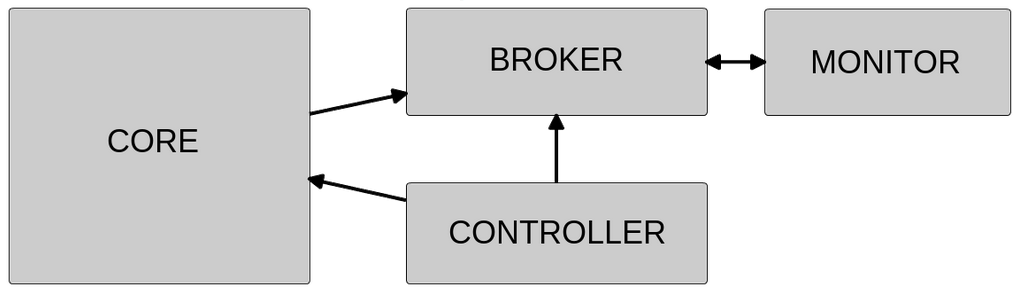
\includegraphics[keepaspectratio = true, width = 400px] {Pictures/nodes}
		\rule{35em}{0.5pt}
	\caption[Struttura]{Struttura ad alto livello.}
	\label{fig:Struttura}
\end{figure}

Come si evince dall'immagine, l'architettura del simulatore è stata divisa in quattro parti:
\begin{itemize}
 \item \textbf{Core}: esegue la simulazione vera e propria, calcolando i tempi, le velocità e tutto ciò che è necessario per lo svolgimento della gara
 \item \textbf{Broker}: riceve gli eventi riguardanti lo svolgimento della gara, li elabora, e li distribuisce agli elementi che ne permettono la visualizzazione ed il controllo da parte dell’utente
 \item \textbf{Monitor}: permette di visualizzare l’andamento della gara tramite una classifica ed una rappresentazione grafica dell’andamento della gara.
 \item \textbf{Controller}: dà la possibilità all’utente di agire come se fosse ai box, indicando al pilota di un veicolo che strategia utilizzare, e pianificando i pit-stop. Permette inoltre di visualizzare dati aggiuntivi sul veicolo.
\end{itemize}


%-----------------------------------
%	SECTION 2
%-----------------------------------
\section{Tipo di comunicazione}

Dopo aver suddiviso il simulatore in componenti che possono essere distribuite su più computer, è stato necessario provvedere alla comunicazione fra quest'ultime.
Si è deciso di prendere in considerazione le seguenti alternative:
\begin{itemize}
\item Utilizzare un middleware
\item Utilizzare una libreria per lo scambio di messaggi (nel caso specifico YAMI4)
\end{itemize}
La prima impone l’architettura del sistema distribuito, fissando i nodi e i ruoli di ogni agente. In questo modo si crea una distribuzione più robusta e definita a priori, che permette l’utilizzo di strutture dati interni al linguaggio in modo condiviso e trasparente.
La seconda, invece, è un insieme di librerie che espongono API che permettono l’invio di messaggi tra le varie entità del sistema distribuito; non viene definita alcuna architettura o nodo, ma viene solo fornito un sistema standard per l’invio e ricezione delle informazioni.
Per quanto la prima soluzione garantisca una maggiore affidabilità, introduce vincoli sul tipo di architettura da implementare ed una intrinseca dipendenza del software dal middleware, con la relativa necessità di installare i vari componenti prima di poter eseguire il programma.
Principalmente per questo motivo, la nostra scelta è ricaduta sulla libreria YAMI4, in quanto ci è sembrato molto importante poter garantire la portabilità di nodi quali il monitor ed il controller, in modo che possano essere avviati su pc in modalità “plug and play”, senza avere la necessità di installare ulteriore software.
Ci siamo resi conto che in una situazione diversa, ad esempio se il nostro software avesse avuto un numero di nodi molto più elevato, sarebbe stato molto rischioso affidarci ad una libreria piuttosto che ad un middleware, proprio per la caratteristica di quest’ultimo di definire ad alto livello l’intero sistema ed i vari ruoli; nel nostro caso però, la scelta di adottare una libreria per lo scambio di messaggi non ha causato problemi.

%-----------------------------------
%	SECTION 3
%-----------------------------------

\section{Comunicazione del Core}

Il core produce sequenza di eventi che indicano il raggiungimento di un obiettivo da parte di un’entità (ad esempio una macchina che esce da un segmento).
Questo flusso di eventi deve essere inviato all’intermediario, per permetterne l’elaborazione e l’invio ai monitor ed i controller.
Il tipo di comunicazione è “uno ad uno”, dato che le istanze del core e dell’intermediario sono uniche; per questo ci è sembrato appropriato utilizzare il metodo push, che permette di inviare ogni nuovo evento con il minimo ritardo possibile.
A differenza del pull, ogni informazione viene spedita, e la frequenza di comunicazione viene gestita dal core. Se la comunicazione fosse stata effettuata direttamente tra il core ed i monitor non sarebbe stato possibile utilizzare questo metodo, visto che ogni monitor non è interessato alla totalità di eventi. Dato che l’intermediario funziona anche come punto di raccolta delle informazioni della gara, siamo sicuri che tutti gli eventi generati dal core saranno di interesse dell’intermediario. Inoltre inviando immediatamente tutte le informazioni disponibili si diminuisce la latenza tra l’istante in cui un evento è generato e quello in cui viene ricevuto ed elaborato.
L’impegno del core dal punto di vista della comunicazione non è limitato unicamente alla trasmissione degli eventi, ma è anche necessario che sia predisposto a ricevere i comandi da parte del controller. Il ragionamento effettuato per la comunicazione core-controller è il medesimo: usando un architettura di tipo pull, sarebbe necessario che il core controllasse in continuazione se qualche giocatore ha inviato un comando, il che aumenterebbe enormemente il carico di lavoro e soprattutto avrebbe esito negativo per la maggior parte delle volte. Per questo è stato utilizzato lo stesso metodo push, ma questa volta dal controller al core (i dettagli del controller verranno descritti successivamente).

%----------------------------------------------------------------------------------------
%	SECTION 4
%----------------------------------------------------------------------------------------

\section{Comunicazione dell’intermediario}

L’intermediario deve poter comunicare su due fronti: ricevere gli eventi dal core, e inviare le informazioni elaborate al monitor ed al controller.
La comunicazione con il core è già stata trattata precedentemente: come spiegato ogni evento viene ricevuto nel modo più rapido possibile.
Dopo aver elaborato le informazioni, bisogna simistarle alle entità monitor e controller, ma la scelta del tipo di comunicazione non è banale.
Ci sono infatti diversi requisiti da soddisfare, in quanto l’intermediario è in possesso di due tipi di informazioni: quelle più generali, che servono a tutti, e quelle più dettagliate, che vengono comunicate su richiesta.
Le tipologie di invio analizzate sono principalmente due, pull e publish subscribe. Nel primo caso le informazioni devono essere recuperate esplicitamente, richiedendole all’intermediario, nel secondo ogni informazioni viene spedita a tutte le entità interessate (che hanno fatto il subscribe).
Ambedue le soluzioni hanno pro e contro, infatti utilizzare il pull implicherebbe una frequenza di aggiornamenti dettata dai monitor, e non dall’arrivo di nuove informazioni, mentre l’utilizzo del publish subscribe comporta l'invio delle informazioni con una cadenza dettata esclusivamente dal produttore.
Entrambe sono utili in determinate circostanze e quindi è stato deciso di adottarle entrambe, utilizzando una per sopperire agli svantaggi dell’altra, e viceversa.
Per questo motivo abbiamo diviso in due parti le informazioni dell’intermediario, quelle che sono necessarie a tutti, e quelle che vengono distribuite su richiesta. Per le prime abbiamo disposto un sistema di publish subscribe che le invia, appena sono disponibili, a tutte le entità registrate per quelle specifiche informazioni; per le seconde abbiamo utilizzato un sistema di pull, creando una risorsa che contiene queste informazioni, e lasciando l’onere di recuperarle all’entità interessata.

%----------------------------------------------------------------------------------------
%	SECTION 5
%----------------------------------------------------------------------------------------

\section{Comunicazione del monitor}

Come detto precedentemente il monitor deve ricevere i dati elaborati dall’intermediario per poter effettuare la rappresentazione grafica.
Tuttavia sono necessari dati aggiuntivi a quelli dell’andamento della gara per poter fare una buona rappresentazione, come ad esempio il numero di partecipanti e di giri, che data la loro staticità durante l’evoluzione non hanno motivo di essere inviati ad ogni publish. Per questo motivo prima di registrarsi alle pubblicazioni dell’intermediario, il monitor recupera in pull queste informazioni aggiuntive tramite la richiesta di un setup.
Completato questo passo la comunicazione continuerà in publish subscribe fino alla fine della gara.

%----------------------------------------------------------------------------------------
%	SECTION 6
%----------------------------------------------------------------------------------------

\section{Comunicazione del Controller}

Il controller permette all’utente di ottenere informazioni aggiuntive riguardo uno specifico veicolo, e offre la possibilità di modificarne le strategie.
La comunicazione si divide quindi in due parti, ricezione dei dati, ed invio.
Riguardo la ricezione viene utilizzato il metodo descritto sopra, e dato che questi dati sono aggiuntivi rispetto a quelli della gara verranno reperiti tramite pull dall’intermediario.
Per l’invio invece, l’idea iniziale è stata quella di inviare le informazioni all’intermediario che si sarebbe poi  occupato di farle arrivare al core. Il problema di questo approccio è dato dal tipo di informazioni che inviamo, infatti a differenza di una semplice visualizzazione grafica che può sopportare una latenza anche di qualche secondo, i dati riguardanti la strategia possono cambiare il corso della gara, ed è quindi necessario farli arrivare al core il prima possibile. Per questo ogni comando dell’utente viene spedito tramite un canale a parte che va dal controller al core, utilizzando il metodo push. In questo modo il core dovrà solo rimanere in ascolto, senza alcun carico di lavoro supplementare. 
Un ulteriore problema può essere causato dal fatto che ciò che vede l’utente dal monitor non è perfettamente in tempo reale, ma soffre di una leggera latenza causata dalla rete e da tutti i calcoli dell’interpolazione dei dati per il rendering grafico. Considerato che i comandi dati dall’utente riguardano esclusivamente la strategia, e non il comportamento immediato del veicolo, siamo giunti alla conclusione che questo non causa un problema nello specifico. Le informazioni sulla strategia infatti non hanno un esecuzione immediata, e quindi possono tranquillamente sopportare una breve latenza.

%----------------------------------------------------------------------------------------
%	SECTION 7
%----------------------------------------------------------------------------------------

\section{Avvio e chiusura del sistema}

Un grosso problema di un sistema distribuito è quello di organizzare l’avvio e la chiusura dell’intero sistema.
Il core e l’intermediario hanno funzioni fortemente correlate, quindi non è stato nemmeno presa in considerazione l’eventualità in cui l’intermediario si possa connettere a gara iniziata
Le situazioni possibili sono due: se durante il bootstrap la comunicazione tra i due va a buon fine, il core lavorerà in modalità distribuita inviando tutti gli eventi all’intermediario man mano che vengono generati; in caso contrario il core eseguirà in modalità locale, consumando gli eventi con delle stampe a schermo degli avvenimenti della gara. Quest’ultima modalità di esecuzione non genera contenuti fruibili per un utente, ed è quindi stata creata solo per motivi di debug.
Quando l’intermediario viene avviato, attende come primo messaggio una comunicazione da parte del core contenente la configurazione della gara. Una volta ricevuto quel messaggio, disporrà le risorse necessarie per permette la comunicazione con il controller ed il monitor.
Questi ultimi due componenti sono stati progettati con l’intento di renderli collegabili e scollegabili a piacere, e possono essere avviati anche a gara iniziata. Questo può essere associato alla realtà con l’idea di poter accendere e spegnerein qualunque momento la TV con cui si guarda la gara o la radio con cui si comunica ai piloti.
Ottenere una chiusura ordinata, invece, ha richiesto l’uso di elementi aggiuntivi. Ogni entità è stata progettata per arrestarsi automaticamente al segnale di chiusura, non forzando l’utente a dover utilizzare CTRL-C o altri comandi di chiusura forzata per terminare l’applicazione.
Quando anche l’ultimo veicolo è arrivato al termine della gara, il core invita ogni task alla chiusura; prima di concludere le attività viene però inviato un evento speciale che indica la conclusione della gara, come ogni evento anche quest’ultimo verrà ricevuto dall’intermediario (per come è stato costruito) che sarà quindi informato del fatto che la gara è terminata. Come per il core, anche l’intermediario comunicherà a tutti i task di cui è composto che la chiusura è imminente.
Il caso del monitor e del controller è leggermente diverso, infatti mentre è auspicabile la chiusura del terminale per il core e l’intermediario, la chiusura improvvisa della finestra di visualizzazione potrebbe non essere altrettanto piacevole per l’utente. In questo caso la terminazione delle altre entità non causerà la chiusura, ma solo una comunicazione all’utente della nuova situazione. A questo punto sarà onere dell’utente chiudere la finestra quando lo riterrà più opportuno, e solo allora il monitor ed il controller si chiuderanno.